%!TEX root = main.tex

\section{StarCraft}
\label{sec:starcrafttheory}


\begin{figure}[h!tb]
\centering
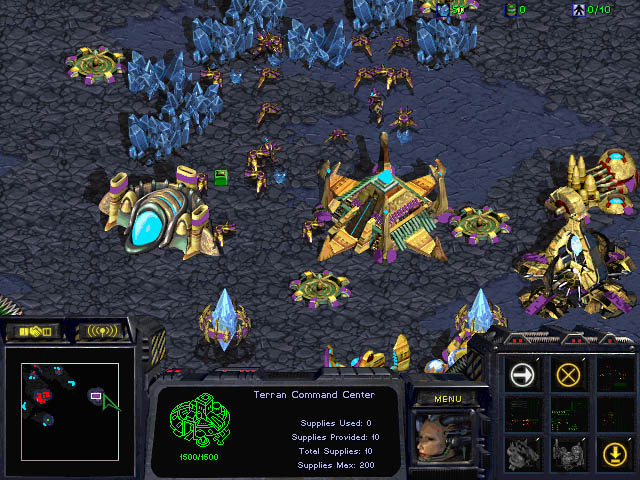
\includegraphics[scale=0.5]{graphics/scbw.jpg}
\caption{StarCraft: Brood War}
\label{fig:scbwIntro}
\end{figure}
%General introduction to the game, with emphasis on the parts that we utilize most in our project

StarCraft is a multi-player, real-time strategy (henceforth referred to as RTS) game, with a heavy focus on both economic strategies, as well as effective management of individual in-game units. Brood War is the expansion pack for the original StarCraft game that introduced new units, maps and upgrades. The game has been praised for its emergent complexity even though the mechanics are simple to understand. StarCraft: Brood War has been played on a high competetive level for over 10 years, and it has been evolving all that time with new strategies and tactics.

\subsection{Races}
The game has three races that a player selects between. The insect-like Zerg, the advanced alien race Protoss and the human
Terrans. Each race has it's own units and buildings as well as different game mechanics. 

\subsubsection{Terran}
\begin{figure}[h!tb]
\centering

\includegraphics[scale=0.6]{graphics/terranicon.png}
\caption{The in-game logo of the Terran race.\cite{terranlogo}}
\end{figure}

The terran are human colonists originally from earth. This is the most balanced race, which relies on a mixture of large numbers and powerful units. They have great mobility in their biological armies, and  great defense and slow turtling in their mechanical units like tanks. 

The Terran worker is a Space Construction Vehicle (SCV), and unique for Terran is that it can repair any mechanical unit or building if they are damaged. Another unique mechanic with Terran is that their buildings can lift off and fly around to reposition themselves.

Several of the buildings can also be upgraded with addons that are smaller buildings that are constructed and connected to the main building. Addons unlock new upgrades and units to be constructed from the building it is connected to. Utilizing the lift off mechanic, buildings can swap addons after they are constructed. This increases the build order diversity, as addons can be switched between construction buildings.

All terran units can be healed after they take damage; the mechanical units and buildings can be repaired using an SCV (but doing so means that the worker will not be gathering resources for that time), and to heal damaged biological units you have to train special units called Medics.

\subsubsection{Zerg}
\begin{figure}[h!tb]
\centering

\includegraphics[scale=0.2]{graphics/zergicon.png}
\caption{The in-game logo of the Zerg race.\cite{zerglogo}}
\end{figure}

The zerg is an insect-like collection of different biological races assimilated under a central intelligence.

They rely on biological abilities that are selectively evolved instead of relying on technology like the other two races.

The individual units in the Zerg army are usually not very powerful, but their strength lies in superior numbers of units as well as the ability to quickly reinforce the army with new units when some die.

The Zerg worker unit is called a drone. What separates this worker from the other races is that in order to create a new building the worker has to ``sacrifice'' itself to morph into the new building, the worker becomes the building.

Zerg has a unique game mechanic for creating new units. The main building, called the hatchery, creates larva on regular intervals, up to a maximum of three, which can be morphed into new units. Both workers and army units are created from the larva, and because of the limited availability on these a player has to prioritize at all times whether he wants to create workers or army units, balancing military strength against economic advantage.

To increase the production capacity they have to either expand to a new base, or create extra support hatcheries in their current bases to gain access to more larva.

Zerg can only build new buildings on creep, a biological substance that covers the ground and spreads from existing buildings as well as from Creep Colonies, a special building that is used only for extending creep coverage on the map.

Zerg units have a unique ability to regenerate health after they are damaged as long as they are not in combat. This makes retreating and regrouping a good tactic for Zerg players as their army will have time to regenerate back to full health after a defeat on the battleground. Together with another unique ability some of the Zerg units have called burrow, which allows them to burrow underground and hide or escape, it can be really hard to kill some units since they can escape and regenerate the lost health. 

\subsubsection{Protoss}
\begin{figure}[h!tb]
\centering

\includegraphics[scale=0.25]{graphics/protossicon.png}
\caption{The in-game logo of the Protoss race.\cite{protosslogo}}
\end{figure}

The protoss is a highly advanced race with powerful mental abilities.

They are both technologically and military advanced, and usually rely on few, but very powerful single units. They have very expensive units that can crush a much bigger army by themselves.

The protoss worker is called a probe, probes doesn't need to construct the buildings, they only tag an area and then the building gets warped in from the protoss home world. This means a single probe can start the construction of several buildings at the same time and then return to gathering resources.

Similar to Zerg, Protoss can't simply construct buildings anywhere, they have to be constructed on a power grid that is generated by pylons, the Protoss supply building.

A unique Protoss feature is that all the units and buildings have shields that protect them from damage and regenerates over time. For an enemy to damage the unit it first has to deplete the shield, then it can do damage to the health of the unit. But damage taken after the shield is down cannot be healed or repaired.

\subsection{Gameplay}
\subsubsection{Micro vs. macro}
Two well-known concepts in the RTS communities, and the StarCraft community in particular, are micro management and macro management. Macro management refers to large-scale economic and strategic decisions, while micro management refers to smaller-scale control of individual units, or groups of units.

A good control of both concepts is needed for a successful agent.

\subsubsection{Supply}
Supply is a term for an artificial limit imposed by the game on how many units a player is allowed to make at any time. To increase the supply, a player can build a special kind of units; for the Protoss race this is {\em pylons}, for Zerg it is {\em overlords} and for Terran it is {\em supply depots}. The name stems from the terran unit needed, supply depots.

\subsubsection{Fog of war and scouting}
Fog of war is a well-known term from RTS games, which denotes un-observed parts of the environment or map. In StarCraft this is shown as shaded on screen. This leads to partial observability, and gives rise to uncertainty about the rest of the map, about what the other player is doing and what resources he has exhausted. To counteract this, it is common to {\em scout}, that is, to send out units to simply observe the other player.

\subsection{BWAPI}
To ease the development of third-party agents that play the game, an application programming interface (API) has been developed for StarCraft: Brood War, by third-party developers. They have relied on reverse engineering of the original game for developing it. It works by injecting itself into the process of the game, and hooking into various functions used in the game, as well as reading various memory areas directly.\cite{bwapi}

There has sprung up a sizable community around this effort, and there are several tournaments where programmers can participate with their own agents.\cite{bwapi}\cite{sscait}

There are also several third-party addons and extra libraries for easing the development of agents, such as the Brood War Terrain Analyzer (BWTA), which provides easy-to-use functions for analyzing the maps for finding choke-points and suitable locations for various buildings,\cite{bwta} and the Brood War Standard Addon Library (BWSAL) which is both a generic, modular framework for BWAPI agents as well as default implementations for a large part of the modules needed for implementing such an agent.\cite{bwsal}

BWAPI only provides a C++ API, so for using it from other languages various types of bindings are needed.\cite{jnibwapi}

There are two modes for loading agents using BWAPI; loading it directly into the StarCraft process, or using a shared-memory area to communicate state between the agent process and the StarCraft process in which the BWAPI code is running.\cite{bwapi}

\subsubsection{JNIBWAPI}
For using Java for developing an agent the most well-supported is using the JNIBWAPI project, which uses JNI to provide Java-bindings for BWAPI. It utilizes the shared-memory approach of BWAPI to avoid having to load the Java virtual machine into the StarCraft memory.
